\section{Natløb}
\subsubsection*{\textbf{Ansvarlig:} \Karla \& \Clint}

Da \karla er kørselsansvarlig, har hun ikke en post, men kan tage billeder, eller evt. assistere, hvor der er brug for det. På dobbeltposterne er der to ansvarlige, som til gengæld også har to poster.

Der gives point til hvert hold i kategorierne Awesomeness, Kampgejst og Bestikkelse på en skala fra 1 til 10, og der gives en samlet bedømmelse som gennemsnittet af disse.

\subsection{Rotationsskema}

\begin{table}[H]
\centering
\begin{tabu}{l *{8}{C{1.4cm}}}\specialrule{1pt}{0pt}{2pt}
\rowfont{\bfseries}
Tid   & Post 1         & Post 2  & Post 3        & Post 4  & Post 5  & Post 6  & Post 7  & Post 8  \\ \specialrule{1pt}{2pt}{2pt}
20:00 & Brasil Ølymp   &         & Skotl Viking  &         & Ægypt   & 'Murica & Austral & Asien   \\ \specialrule{.25pt}{1pt}{1pt}
20:15 & Skotl Asien    &         & Brasil Austral&         & 'Murica & Viking  & Ægypt   & Ølymp   \\ \specialrule{.25pt}{1pt}{1pt}
20:30 & Viking 'Murica &         & Ølymp Ægypt   &         & Brasil  & Skotl   & Asien   & Austral \\ \specialrule{.25pt}{1pt}{1pt}
20:45 & Austral Ægypt  &         & Asien 'Murica &         & Skotl   & Ølymp   & Viking  & Brasil  \\ \specialrule{.25pt}{1pt}{1pt}
21:00 &         & Brasil Asien   &        & 'Murica Ægypt  & Ølymp   & Austral & Skotl   & Viking  \\ \specialrule{.25pt}{1pt}{1pt}
21:15 &         & Ølymp Viking   &        & Brasil Skotl   & Austral & Asien   & 'Murica & Ægypt   \\ \specialrule{.25pt}{1pt}{1pt}
21:30 &         & Skotl Ægypt    &        & Viking Austral & Asien   & Brasil  & Ølymp   & 'Murica \\ \specialrule{.25pt}{1pt}{1pt}
21:45 &         & 'Murica Austral&        & Ølymp Asien    & Viking  & Ægypt   & Brasil  & Skotl   \\ \specialrule{1pt}{2pt}{0pt}
\end{tabu}
\end{table}

\begin{table}[H]
\caption{\underline{Point på post:\qquad \qquad \qquad \qquad \qquad}}
\label{tab:natløb_point_01}
\centering
\begin{tabu}{L{3.5cm} *{4}{|C{2.5cm}}}\specialrule{1pt}{0pt}{2pt}
\rowfont{\bfseries}
Hold & Awesomeness & Kampgejst & Bestikkelse & Samlet \\ \specialrule{1pt}{2pt}{2pt}
Brasilien       & & & & \\ \specialrule{.25pt}{1pt}{1pt}
Ølympen         & & & & \\ \specialrule{.25pt}{1pt}{1pt}
Skotland        & & & & \\ \specialrule{.25pt}{1pt}{1pt}
Sydøstasien     & & & & \\ \specialrule{.25pt}{1pt}{1pt}
Vikingeland     & & & & \\ \specialrule{.25pt}{1pt}{1pt}
'Murica!        & & & & \\ \specialrule{.25pt}{1pt}{1pt}
Australien      & & & & \\ \specialrule{.25pt}{1pt}{1pt}
Ægypten         & & & & \\ \specialrule{1pt}{2pt}{0pt}
\end{tabu}
\end{table}

\begin{table}[H]
\caption{\underline{Point på post:\qquad \qquad \qquad \qquad \qquad}}
\label{tab:natløb_point_02}
\centering
\begin{tabu}{L{3.5cm} *{4}{|C{2.5cm}}}\specialrule{1pt}{0pt}{2pt}
\rowfont{\bfseries}
Hold & Awesomeness & Kampgejst & Bestikkelse & Samlet \\ \specialrule{1pt}{2pt}{2pt}
Brasilien       & & & & \\ \specialrule{.25pt}{1pt}{1pt}
Ølympen         & & & & \\ \specialrule{.25pt}{1pt}{1pt}
Skotland        & & & & \\ \specialrule{.25pt}{1pt}{1pt}
Sydøstasien     & & & & \\ \specialrule{.25pt}{1pt}{1pt}
Vikingeland     & & & & \\ \specialrule{.25pt}{1pt}{1pt}
'Murica!        & & & & \\ \specialrule{.25pt}{1pt}{1pt}
Australien      & & & & \\ \specialrule{.25pt}{1pt}{1pt}
Ægypten         & & & & \\ \specialrule{1pt}{2pt}{0pt}
\end{tabu}
\end{table}


\subsection{Posterne}

\subsubsection*{Oversigt}
\begin{enumerate}
  \item Jorden af lava - \stive\& \buddha - Gårdsplads
  \item Klemme-limbo - \stive\& \buddha - Spisesalen
  \item Puste lys ud - \clint\& \farav - Pejsestuen
  \item Forme trylledej - \clint\& \farav - Pejsestuen
  \item Spider web - \randildo - Rusværelse (Uddeles på turen)
  \item Risk-puslespil - \hemorides - Gang ved siden af "Kongressen"
  \item Strøm 1 - \mighty - Plæne foran køkken
  \item Frugtvektorer - \Hyttebums{Bumz} - Sal foran køkken
\end{enumerate}

\subsubsection*{Post 1 - Jorden af lava}

\textbf{Ansvarlig:} \Stive \& \Buddha

\textbf{Historien:} I er på en tropisk vulkan-ø, og vulkanen er gået i udbrud. I skal væk ASAP, og har kun de lava-resistente ølkasser til at flygte på.

\textbf{Legen:} Der laves en kombineret start/mål-streg med gaffatape. Hvert hold skal fra start, rundt om en udfordring (et bord etc.) og så i mål, uden at røre jorden, ved flytte ølkasser fra bagerste til forreste mand. Det hold der først har alle mand over målstregen vinder. Hvis man rører jorden undervejs, er man død, og starter forfra.

\textbf{Materialer:}
\begin{itemize}
  \item 8 ølkasser/mælkekasser (4 kasser pr. hold, dvs. kunne stå på tre og flytte den fjerde)
  \item Gaffatape
\end{itemize}

\begin{table}[H]
\begin{tabu}{*{3}{l}}\specialrule{1pt}{0pt}{2pt}
\rowfont{\bfseries}
Starttid & Hold til stede & Sendes videre til \\ \specialrule{1pt}{2pt}{2pt}
20:00 & Brasilien   & Puste lys ud i pejsestuen hos \clint og \farav                \\ \specialrule{.25pt}{1pt}{1pt}
20:00 & Ølympen     & Frugtvektorer i salen foran køkkenet hos \Hyttebums{Piraterne}\\ \specialrule{.25pt}{1pt}{1pt}
20:15 & Skotland    & Risk-puslespil på gangen ved "Kongressen" hos \hemorides      \\ \specialrule{.25pt}{1pt}{1pt}
20:15 & Sydøstasien & Strøm 1 på plænen foran køkkenet hos \mighty                  \\ \specialrule{.25pt}{1pt}{1pt}
20:30 & Vikingeland & Strøm 1 på plænen foran køkkenet hos \mighty                  \\ \specialrule{.25pt}{1pt}{1pt}
20:30 & 'Murica!    & Puste lys ud i pejsestuen hos \clint og \farav                \\ \specialrule{.25pt}{1pt}{1pt}
20:45 & Australien  & Risk-puslespil på gangen ved "Kongressen" hos \hemorides      \\ \specialrule{.25pt}{1pt}{1pt}
20:45 & Ægypten     & Trylledej i pejsestuen hos \clint og \farav                   \\ \specialrule{1pt}{2pt}{0pt}
\end{tabu}
\end{table}

\subsubsection*{Post 2 - Klemme-limbo}

\textbf{Ansvarlig:} \Stive \& \Buddha

\textbf{Historien:} I enhver krig er det vigtigt at være smidig, for at kunne undgå fjendens kugler (ligesom under sex). Derfor skal vi nu træne smidighed ved at lege klemme-limbo.

\textbf{Legen:} Man skal med munden montere en tøjklemme på en tørresnor. Næste holdkammerat skal så med munden sætte en klemme på den første tøjklemme, og det gælder således om at lave den længste kæde af tøjklemmer, ved kun at bruge munden. Man går frem ligesom i limbo - hænderne må ikke røre jorden/gulvet (Evt. hjælp fra holdkammerater kan godkendes).

\textbf{Materialer:}
\begin{itemize}
  \item 40 træklemmer
  \item 4 m tørresnor
\end{itemize}

\begin{table}[H]
\begin{tabu}{*{3}{l}}\specialrule{1pt}{0pt}{2pt}
\rowfont{\bfseries}
Starttid & Hold til stede & Sendes videre til \\ \specialrule{1pt}{2pt}{2pt}
21:00 & Brasilien   & Trylledej i pejsestuen hos \clint og \farav                   \\ \specialrule{.25pt}{1pt}{1pt}
21:00 & Sydøstasien & Risk-puslespil på gangen ved "Kongressen" hos \hemorides      \\ \specialrule{.25pt}{1pt}{1pt}
21:15 & Ølympen     & Strøm 1 på plænen foran køkkenet hos \mighty                  \\ \specialrule{.25pt}{1pt}{1pt}
21:15 & Vikingeland & Trylledej i pejsestuen hos \clint og \farav                   \\ \specialrule{.25pt}{1pt}{1pt}
21:30 & Skotland    & Frugtvektorer i salen foran køkkenet hos \Hyttebums{Piraterne}\\ \specialrule{.25pt}{1pt}{1pt}
21:30 & Ægypten     & Risk-puslespil på gangen ved "Kongressen" hos \hemorides      \\ \specialrule{.25pt}{1pt}{1pt}
21:45 & 'Murica!    &                                                               \\ \specialrule{.25pt}{1pt}{1pt}
21:45 & Australien  &                                                               \\ \specialrule{1pt}{2pt}{0pt}
\end{tabu}
\end{table}

\subsubsection*{Post 3 - Puste lys ud}

\textbf{Ansvarlig:} \Clint \& \Farav

\textbf{Historien:} Det er krisetider! Der er meget begrænsede madforsyninger, så det gælder om at være hurtig, hvis man ikke vil gå sulten i seng. For at spise, skal man kunne se hvad man spiser, og man må derfor kun spise, når ens lys er tændt, og hvis man ikke vil have de andre spiser det sidste mad, må man sørge for de ikke har lys.

\textbf{Legen:} To fra hvert hold starter med at dyste mod hinanden. Man sætter sig overfor modstanderholdet, og hver deltager udstyres med et lys, en lighter og en bunke kiks. Det gælder om først at komme igennem sine kiks, men man må kun spise, så længe der er ild i ens eget lys, og man må puste modstanderens lys ud det bedste man har lært.

\textbf{Materialer:}
\begin{itemize}
  \item 300 stk marie kiks
  \item 10 fyrfadslys
  \item 15 lightere
\end{itemize}

\begin{table}[H]
\begin{tabu}{*{3}{l}}\specialrule{1pt}{0pt}{2pt}
\rowfont{\bfseries}
Starttid & Hold til stede & Sendes videre til \\ \specialrule{1pt}{2pt}{2pt}
20:00 & Skotland    & Jorden af lava på gårdspladsen hos \stive og \buddha          \\ \specialrule{.25pt}{1pt}{1pt}
20:00 & Vikingeland & Risk-puslespil på gangen ved "Kongressen" hos \hemorides      \\ \specialrule{.25pt}{1pt}{1pt}
20:15 & Brasilien   & Spider web på rusværelset hos \randildo                       \\ \specialrule{.25pt}{1pt}{1pt}
20:15 & Australien  & Frugtvektorer i salen foran køkkenet hos \Hyttebums{Piraterne}\\ \specialrule{.25pt}{1pt}{1pt}
20:30 & Ølympen     & Risk-puslespil på gangen ved "Kongressen" hos \hemorides      \\ \specialrule{.25pt}{1pt}{1pt}
20:30 & Ægypten     & Jorden af lava på gårdspladsen hos \stive og \buddha          \\ \specialrule{.25pt}{1pt}{1pt}
20:45 & Sydøstasien & Klemme-limbo i spisesalen hos \stive og \buddha               \\ \specialrule{.25pt}{1pt}{1pt}
20:45 & 'Murica!    & Trylledej i pejsestuen hos \clint og \farav                   \\ \specialrule{1pt}{2pt}{0pt}
\end{tabu}
\end{table}

\subsubsection*{Post 4 - Forme trylledej}

\textbf{Ansvarlig:} \Clint \& \Farav

\textbf{Historien:} Når man er ude for at erobre lande, kan det være en stor fordel at kunne kommunikere med folk, der taler andre sprog. Derfor skal I træne at udtrykke forskellige ord i trylledej.

\textbf{Legen:} Hvert hold får udleveret en klump trylledej, og skal så forme forskellige ting i dejen. Det ene hold får rigtig nemme opgaver, og det andet hold får rigtig svære opgaver. Det er tilladt at placere dej på kroppen. F.eks. kan en fingerring placeres på fingeren. Det er ikke tilladt at forme tal eller bogstaver, samt at lave fagter eller sige noget.

\textbf{Materialer:}
\begin{itemize}
  \item 3 L mel
  \item 1,5 L salt
  \item 1,5 L vand
  \item 2-3 dL madolie
  \item Lister med nemme og svære opgaver
  \item Kuglepen (til at skrive med \Hashtag{Logik?})
\end{itemize}

\begin{table}[H]
\begin{tabu}{*{3}{l}}\specialrule{1pt}{0pt}{2pt}
\rowfont{\bfseries}
Starttid & Hold til stede & Sendes videre til \\ \specialrule{1pt}{2pt}{2pt}
21:00 & 'Murica!    & Strøm 1 på plænen foran køkkenet hos \mighty                  \\ \specialrule{.25pt}{1pt}{1pt}
21:00 & Ægypten     & Frugtvektorer i salen foran køkkenet hos \Hyttebums{Piraterne}\\ \specialrule{.25pt}{1pt}{1pt}
21:15 & Brasilien   & Risk-puslespil på gangen ved "Kongressen" hos \hemorides      \\ \specialrule{.25pt}{1pt}{1pt}
21:15 & Skotland    & Klemme-limbo i spisesalen hos \stive og \buddha               \\ \specialrule{.25pt}{1pt}{1pt}
21:30 & Vikingeland & Spider web på rusværelset hos \randildo                       \\ \specialrule{.25pt}{1pt}{1pt}
21:30 & Australien  & Klemme-limbo i spisesalen hos \stive og \buddha               \\ \specialrule{.25pt}{1pt}{1pt}
21:45 & Ølympen     &                                                               \\ \specialrule{.25pt}{1pt}{1pt}
21:45 & Sydøstasien &                                                               \\ \specialrule{1pt}{2pt}{0pt}
\end{tabu}
\end{table}
Husk at være nogle champs og gem trylledejen (i en lukket pose), så den kan genbruges til Dameaften \Hashtag{GenbrugErBedstForAlle}. 

\begin{minipage}{0.5\textwidth}
\textbf{De nemme}
\begin{itemize}
\item Dej
\item Bold
\item Sol
\item Penis
\item Trekant
\item Kop
\item Terning
\item Hjul
\item Saks
\item Bord
\item Kors
\item Armbånd
\item Bøjle
\item Briller
\item Stige
\item Flag
\item Sko
\item Vindmølle
\item Sut
\item Slikkepind
\item Snemand
\item Anker
\item Lup
\item Pistol
\item Gevær 
\item Sværd
\item Økse
\item Stjerne
\item Edderkop
\item Kam
\item Gaffel 
\item Båd
\item Bro
\item Vulkan
\item Palme
\item Måne
\item Fugl
\item Blomst
\item Bog
\item Nøgle
\item Fisk
\item Legoklods
\item Stok
\item Krone
\item Clips
\item Horn
\item Pil
\item Flaske
\item Lasso
\item Pølse
\end{itemize}
\end{minipage}
\begin{minipage}{0.5\textwidth}
\textbf{De svære}
\begin{itemize}
\item Big Bang
\item Optimisme
\item Forår
\item Magtens tredeling
\item Storebælt
\item Passatvinden
\item Forkert
\item Middelmådig
\item Frustration
\item Tre fjerdedele
\item Friværdi
\item Bagerjomfru
\item Egenkapital
\item Håndskrift
\item Savl
\item Længdespring
\item Futurisme
\item Hånefuld
\item Tømmermænd
\item Døv
\item Fortvivlelse
\item Minimalisme
\item Ferie
\item Modersmål
\item Biograf
\item Klaustrofobi
\item Krigsførelse
\item Slaget ved Waterloo
\item Marianergraven
\item Oase
\item Grønlænder
\item Nederlag
\item Sejr
\item Frankrig
\item Nynazisme
\item Gravad Laks
\item Surstrømninger
\item Diarré
\item Søsyge 
\item Harem
\item Spork 
\item Søpapegøje 
\item Autoritet
\item Humanisme
\item Naturvidenskab
\item Eksistentialisme 
\item Tidsfordriv
\item Underernæring
\item Arbejdsløshed
\end{itemize}
\end{minipage}

\subsubsection*{Post 5 - Spider web}

\textbf{Ansvarlig:} \Randildo

\textbf{Historien:} I er på hemmelig mission over fjendens linjer og trængt ind i deres hovedkvarter. For at få fat i koderne til missilprogrammet, skal i trænge forbi lasersensorerne, uden at aktivere alarmen!

\textbf{Legen:} Det gøres selvfølgelig ved fælles hjælp at få flest personer gennem spindelvævet af snore, uden at røre linjerne. Des sværere hul, des flere point og jo flere I får igennem på tid, jo flere point. Alle skal igennem (man må ikke bare vælge den mindste og flytte vedkommende frem og tilbage).

\textbf{Materialer:}
\begin{itemize}
  \item 20 m snor
\end{itemize}

\begin{table}[H]
\begin{tabu}{*{3}{l}}\specialrule{1pt}{0pt}{2pt}
\rowfont{\bfseries}
Starttid & Hold til stede & Sendes videre til \\ \specialrule{1pt}{2pt}{2pt}
20:00 & Ægypten     & Strøm 1 på plænen foran køkkenet hos \mighty                  \\ \specialrule{.25pt}{1pt}{1pt}
20:15 & 'Murica!    & Jorden af lava på gårdspladsen hos \stive og \buddha          \\ \specialrule{.25pt}{1pt}{1pt}
20:30 & Brasilien   & Frugtvektorer i salen foran køkkenet hos \Hyttebums{Piraterne}\\ \specialrule{.25pt}{1pt}{1pt}
20:45 & Skotland    & Strøm 1 på plænen foran køkkenet hos \mighty                  \\ \specialrule{.25pt}{1pt}{1pt}
21:00 & Ølympen     & Klemme-limbo i spisesalen hos \stive og \buddha               \\ \specialrule{.25pt}{1pt}{1pt}
21:15 & Australien  & Trylledej i pejsestuen hos \clint og \farav                   \\ \specialrule{.25pt}{1pt}{1pt}
21:30 & Sydøstasien & Trylledej i pejsestuen hos \clint og \farav                   \\ \specialrule{.25pt}{1pt}{1pt}
21:45 & Vikingeland &                                                               \\ \specialrule{1pt}{2pt}{0pt}
\end{tabu}
\end{table}

\subsubsection*{Post 6 - Risk-puslespil}

\textbf{Ansvarlig:} \Hemorides 

\textbf{Historien:} Når man sejler på de syv verdenshave, er det en fordel at kende verdenskortet. 

\textbf{Legen:} Derfor skal I nu placere så mange lande som muligt, korrekt, på Riskpladen. I får \Hashtag{sex} minutter til det.

\textbf{Materialer:}
\begin{itemize}
  \item Risk-plade (hjemmeprintet A2, tapet til bord)
  \item Lande-labels (2 sæt, lamineret)
  \item RISK-kort med rigtig svar
% \item Elefant snot % ligegyldig?
\end{itemize}

\begin{table}[H]
\begin{tabu}{*{3}{l}}\specialrule{1pt}{0pt}{2pt}
\rowfont{\bfseries}
Starttid & Hold til stede & Sendes videre til \\ \specialrule{1pt}{2pt}{2pt}
20:00 & 'Murica!    & Spider web på rusværelset hos \randildo                       \\ \specialrule{.25pt}{1pt}{1pt}
20:15 & Vikingeland & Jorden af lava på gårdspladsen hos \stive og \buddha          \\ \specialrule{.25pt}{1pt}{1pt}
20:30 & Skotland    & Spider web på rusværelset hos \randildo                       \\ \specialrule{.25pt}{1pt}{1pt}
20:45 & Ølympen     & Spider web på rusværelset hos \randildo                       \\ \specialrule{.25pt}{1pt}{1pt}
21:00 & Australien  & Spider web på rusværelset hos \randildo                       \\ \specialrule{.25pt}{1pt}{1pt}
21:15 & Sydøstasien & Spider web på rusværelset hos \randildo                       \\ \specialrule{.25pt}{1pt}{1pt}
21:30 & Brasilien   & Strøm 1 på plænen foran køkkenet hos \mighty                  \\ \specialrule{.25pt}{1pt}{1pt}
21:45 & Ægypten     &                                                               \\ \specialrule{1pt}{2pt}{0pt}
\end{tabu}
\end{table}

\begin{figure}[H]
\begin{center}
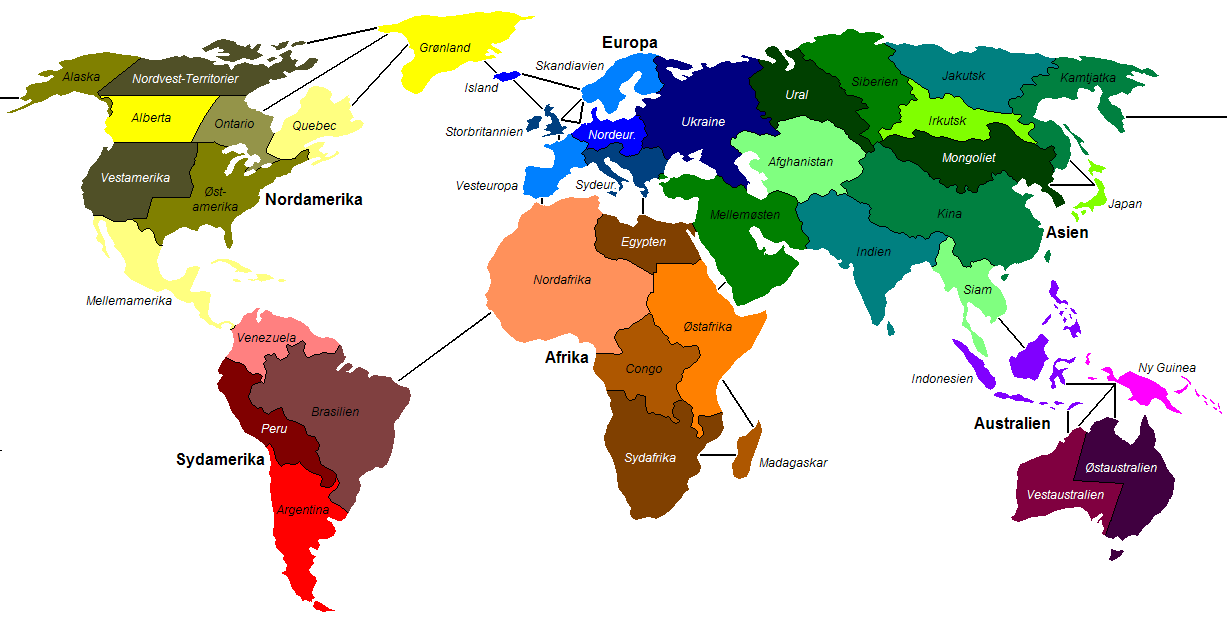
\includegraphics[width=\textwidth]{fig/RISKplade.png}
\end{center}
\end{figure}


\subsubsection*{Post 7 - Introduktion til Strømningsmekanik 1 \Hashtag{LigesomUnderSex}}

\textbf{Ansvarlig:} \Mighty

\textbf{Historien:} Vores vandressourcer er ved at slippe op, og vi skal derfor have transporteret mest muligt vand på kort tid. Det ærgerlige er, at da I alle har mistet jeres arme under krig, er I nødt til at flytte det med munden. Denne øvelse er samtidig en god introduktion til Strømningsmekanik 1, til de af jer, der skal have det.

\textbf{Legen:} Vand skal flyttes fra én balge til en anden. Den første rus må gerne bruge hænder til at fylde sin kop, inden personen tager den i munden (ligesom under sex). Derefter skal kruset sendes fra mund til mund ned til den sidste i rækken, som så hælder det i baljen.

\textbf{Materialer:}
\begin{itemize}
  \item 2 baljer
  \item 100 engangskrus (med kant, så de kan holdes med tænderne)
  \item Vand
\end{itemize}

\begin{table}[H]
\begin{tabu}{*{3}{l}}\specialrule{1pt}{0pt}{2pt}
\rowfont{\bfseries}
Starttid & Hold til stede & Sendes videre til \\ \specialrule{1pt}{2pt}{2pt}
20:00 & Australien  & Puste lys ud i pejsestuen hos \clint og \farav                \\ \specialrule{.25pt}{1pt}{1pt}
20:15 & Ægypten     & Puste lys ud i pejsestuen hos \clint og \farav                \\ \specialrule{.25pt}{1pt}{1pt}
20:30 & Sydøstasien & Puste lys ud i pejsestuen hos \clint og \farav                \\ \specialrule{.25pt}{1pt}{1pt}
20:45 & Vikingeland & Frugtvektorer i salen foran køkkenet hos \Hyttebums{Piraterne}\\ \specialrule{.25pt}{1pt}{1pt}
21:00 & Skotland    & Trylledej i pejsestuen hos \clint og \farav                   \\ \specialrule{.25pt}{1pt}{1pt}
21:15 & 'Murica!    & Frugtvektorer i salen foran køkkenet hos \Hyttebums{Piraterne}\\ \specialrule{.25pt}{1pt}{1pt}
21:30 & Ølympen     & Trylledej i pejsestuen hos \clint og \farav                   \\ \specialrule{.25pt}{1pt}{1pt}
21:45 & Brasilien   &                                                               \\ \specialrule{1pt}{2pt}{0pt}
\end{tabu}
\end{table}

\subsubsection*{Post 8 - Frugtvektorer}

\textbf{Ansvarlig:} \Hyttebums{Hyttebumz}

\textbf{Historien:} I er netop ankommet til et vestligt land, hvor maden er i overflod og beskæftigelsen i bund. Kunst er den nye levevej (\Hashtag{RUC}) og det skal helst være kortvarigt og sært (\Hashtag{HverdagsSM}). I skal derfor bygge jeres tværvektor ud af frugter.

\textbf{Legen:} Byg jeres tværvektor i frugt

\textbf{Materialer:}
\begin{itemize}
  \item 4 Agurker
  \item Klementiner
  \item Tændstikker
  \item Grillspydpinde
  \item 2 sorte tuscher
\end{itemize}

\begin{table}[H]
\begin{tabu}{*{3}{l}}\specialrule{1pt}{0pt}{2pt}
\rowfont{\bfseries}
Starttid & Hold til stede & Sendes videre til \\ \specialrule{1pt}{2pt}{2pt}
20:00 & Sydøstasien & Jorden af lava på gårdspladsen hos \stive og \buddha          \\ \specialrule{.25pt}{1pt}{1pt}
20:15 & Ølympen     & Puste lys ud i pejsestuen hos \clint og \farav                \\ \specialrule{.25pt}{1pt}{1pt}
20:30 & Australien  & Jorden af lava på gårdspladsen hos \stive og \buddha          \\ \specialrule{.25pt}{1pt}{1pt}
20:45 & Brasilien   & Klemme-limbo i spisesalen hos \stive og \buddha               \\ \specialrule{.25pt}{1pt}{1pt}
21:00 & Vikingeland & Klemme-limbo i spisesalen hos \stive og \buddha               \\ \specialrule{.25pt}{1pt}{1pt}
21:15 & Ægypten     & Klemme-limbo i spisesalen hos \stive og \buddha               \\ \specialrule{.25pt}{1pt}{1pt}
21:30 & 'Murica!    & Klemme-limbo i spisesalen hos \stive og \buddha               \\ \specialrule{.25pt}{1pt}{1pt}
21:45 & Skotland    &                                                               \\ \specialrule{1pt}{2pt}{0pt}
\end{tabu}
\end{table}
